\section{Cornershop viral}

Una importante empresa de reparto de productos a domicilio Cornershop ha tenido mucha demanda por los últimos casos de COVID19 y todo el alboroto que ha generado ultimamente en los supermercados locales, se le pide ayuda a usted, un programador excelente, que ayude a controlar todo el desorden por el sobrecolapso que se generó en la empresa y poder recibir todos los pedidos de esta gente \sout{alarmista} desabastecida.

%\sout{tachar} \emph{enfasis}
Se tienen dos archivos de texto \texttt{precios.txt} y \texttt{pedidos.txt}. 

\begin{figure}[H]
    \centering
    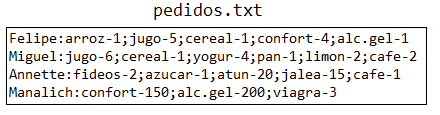
\includegraphics{Imagenes/pedidos.png}
\end{figure}
\begin{figure}[H]
    \centering
    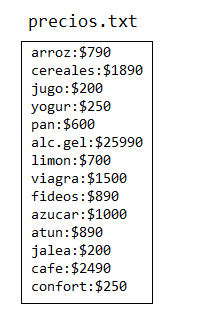
\includegraphics{Imagenes/precios.png}
\end{figure}

\begin{itemize}
    \item \texttt{precios.txt} contiene la información de los precios de los productos disponibles, donde cada línea tiene el formato \texttt{producto:\$precio} en pesos chilenos. 
    \item \texttt{pedidos.txt} contiene la información de los pedidos diarios donde el formato de cada línea es \texttt{nombre:producto1-cantidad1;producto2-cantidad2;...}, donde los productos están separados por puntos y coma, estos a su vez tienen los datos del producto y la cantidad separadas por guión.
\end{itemize}

Se le pide a usted generar archivos de texto referentes a las boletas de cada usuario que tengan la siguiente información
\begin{itemize}
    \item Nombre del usuario al principio del archivo
    \item Detalle de cada compra que incluye 
    \begin{itemize}
        \item Nombre del producto: \textbf{Producto}
        \item Cantidad: \textbf{Cantidad}
        \item Precio unitario: \textbf{P. unitario}
        \item Total: \textbf{Total}
    \item El total de la compra
    \end{itemize}
\end{itemize}

\begin{figure}[H]
    \centering
    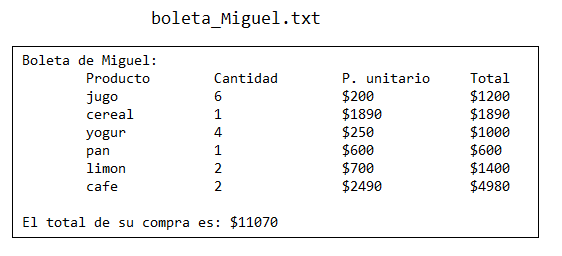
\includegraphics{Imagenes/boletamia.png}
\end{figure}

Para esto ayúdese programando las siguientes funciones
\begin{itemize}
    \item[a.] \texttt{buscar\_precio(producto,precios)} que reciba como parámetros un string con el producto a buscar su precio y el nombre del archivo con los precios. Esta función retorna un entero con el precio del producto, en caso de que no se encuentre el producto en el archivo de precios, esta función retorna \texttt{False}.
    \begin{lstlisting}[style=consola]
>>> [*buscar_precio('alc.gel','precios.txt')*]
25990
    \end{lstlisting}
    \item[b.] \texttt{diccionario\_pedido(linea\_pedido)} que reciba un string con las líneas de los pedidos, en este caso un string separado por puntos y coma de la forma \texttt{producto1-cantidad1;producto2-cantidad2;...}. Esta función retorna un diccionario donde sus llaves son los productos y sus valores son la cantidad en formato entero.
\begin{lstlisting}[style=consola]
[*>>> diccionario_pedido('fideos-2;azucar-1;atun-20;jalea-15;cafe-1')*]
{'fideos': 2, 'azucar': 1, 'atun': 20, 'jalea': 15, 'cafe': 1}
\end{lstlisting}
    
    \item[c.] \texttt{crear\_archivos(precios,pedidos)} que reciba como parámetros los nombres de los dos archivos de texto iniciales, esta función debe escribir un archivo de texto por cada línea de pedido con el nombre \texttt{boleta\_Usuario.txt}, donde \texttt{Usuario} es el nombre del personaje que hace el pedido. Para los formatos de las líneas guíese de los siguientes strings a interpolar con el método format.
    \begin{lstlisting}[style=consola]
Nombre del archivo:     [*'boleta_{}.txt'*]
Primera linea:          [*'Boleta de {}:\n'*]
Titulo detalle:         [*'\tProducto\tCantidad\tP. unitario\tTotal\n'*]
Linea de cada producto: [*'\t{0}\t\t{1}\t\t${2}\t\t${3}\n'*]
Linea final de boleta:  [*'\nEl total de su compra es: ${}'*]
    \end{lstlisting}
    Esta función retorna nada.
\end{itemize}

